\section{Цель работы}
Цель работы --- решить задачу интерполяции, найти значения функции при
заданных значениях аргумента, отличных от узловых точек
\section{Рабочие формулы используемых методов}
\begin{itemize}
  \item Многочлен Лагранжа
    \[ L_n(x) = \sum_{i = 0}^n y_i \prod_{j=0; j \neq i} \frac{x - x_j}{x_i - x_j} \]
  \item Многочлен Ньютона с разделенными разностями
    \[ 
    N_n(x) = f(x_0) + \sum_{k = 1}^n f(x_0, x_1, \ldots, x_k)
    \prod_{j=0}^{k-1} (x - x_j)
    \]
  \item Многочлен Ньютона с конечными разностями, интерполирование вперед
    \[
      t = (x - x_0) / h \qquad
    N_n(x) = y_0 + t \Delta y_0 + \frac{t(t-1)}{2!} \Delta^2 y_0
    + \cdots + \frac{t(t-1)\cdots(t-n+1)}{n!} \Delta^n y_0
    \]
\end{itemize}

\section{Вычислительная часть задачи}
Значения функции \(y = f(x)\) представлены на~\cref{tab:function}.
\(x_1 = 0.534\), \(x_2 = 0.384\).
Таблица конечных разностей представлена на~\cref{tab:finite_dif}.
Для вычисления \(x_1\) воспользуемся интерполированием назад.
Тогда \( t = (x - x_n) / h = (0.534 - 0.55) / 0.05 = -0.32 \)
\begin{table}
  \caption{Значения функции \(y = f(x)\)}\label{tab:function}
  \centering
  \begin{tabular}{rr}
    \toprule
    \(x\) & \(y\) \\
    \midrule
    0.25 & 1.2557 \\
    0.30 & 2.1764 \\
    0.35 & 3.1218 \\
    0.40 & 4.0482 \\
    0.45 & 5.9875 \\
    0.50 & 6.9195 \\
    0.55 & 7.8359 \\
    \bottomrule
  \end{tabular}
\end{table}

\begin{align*}
  N(x) &= y_6 + t \Delta y_5 + t(t+1)/2 \Delta^2 y_4 + t(t+1)(t+2)/6 \Delta^3 y_3 + t(t+1)(t+2)(t+3)/24 \Delta^4 y_2 + \\ &+ t(t+1)(t+2)(t+3)(t+4)/120 \Delta^5 y_1 + 
  t(t+1)(t+2)(t+3)(t+4)(t+5)/720 \Delta^6 y_0 = \\
  &= 7.8359 -0.29 + 0.00 -0.06 -0.12 -0.18 -0.24 = \\
  &= 6.9399
\end{align*}

\begin{table}
  \caption{Значения конченых разностей}\label{tab:finite_dif}
  \centering
  \begin{tabular}{rrrrrrrr}
    \toprule
      \(y_i = \Delta^0 y_i\)
    & \(\Delta y_i\)
    & \(\Delta^2 y_i\)
    & \(\Delta^3 y_i\)
    & \(\Delta^4 y_i\)
    & \(\Delta^5 y_i\)
    & \(\Delta^6 y_i\) \\
    \midrule
    +1.2557  &      +0.9207 &       +0.0247 &       -0.0437 &       +1.0756 &       -4.1277 &       +10.1917 \\
    +2.1764  &      +0.9454 &       -0.0190 &       +1.0319 &       -3.0521 &       +6.0640 & -- \\
    +3.1218  &      +0.9264 &       +1.0129 &       -2.0202 &       +3.0119 & -- & -- \\
    +4.0482  &      +1.9393 &       -1.0073 &       +0.9917 & -- & -- & -- \\
    +5.9875  &      +0.9320 &       -0.0156 & -- & -- & -- & -- \\
    +6.9195  &      +0.9164 & -- & -- & -- & -- & -- \\
    +7.8359  &  -- & -- & -- & -- & -- & -- \\

    \bottomrule
  \end{tabular}
\end{table}

Теперь вычислим значение \(X_2 = 0.384 \)
Возьмем \(x_0 = a = 0.4 \).
Т.к. \(X_2 = 0.384 < a \), то воспользуемся
второй интерполяционной формулой Гаусса.

\begin{align*}
  P(x) &=
  y_0 + t \Delta y_{-1} + \frac{t(t+1)}{2!} \Delta^2 y_{-1}
  + \frac{t(t+1)t(t-1)}{3!} \Delta^3 y_{-2} +
  \frac{(t+2)(t+1)t(t-1)}{4!} \Delta^4 y_{-2} + \\
  &+ \frac{t(t+1)(t-1)(t+2)(t-2)} \Delta^5 y_{-3}
  \frac{t(t+1)(t-1)(t+2)(t-2)(t-3)} \Delta^6 y_{-3} = \\
  &= 4.048  -0.296  -0.110 + 0.049  -0.061 + 0.039  -0.042 = \\
  &= 3.626
\end{align*}

\section{Программная часть задачи}
\inputminted[breaklines]{Python}{../solution/solution.py}

\begin{center}
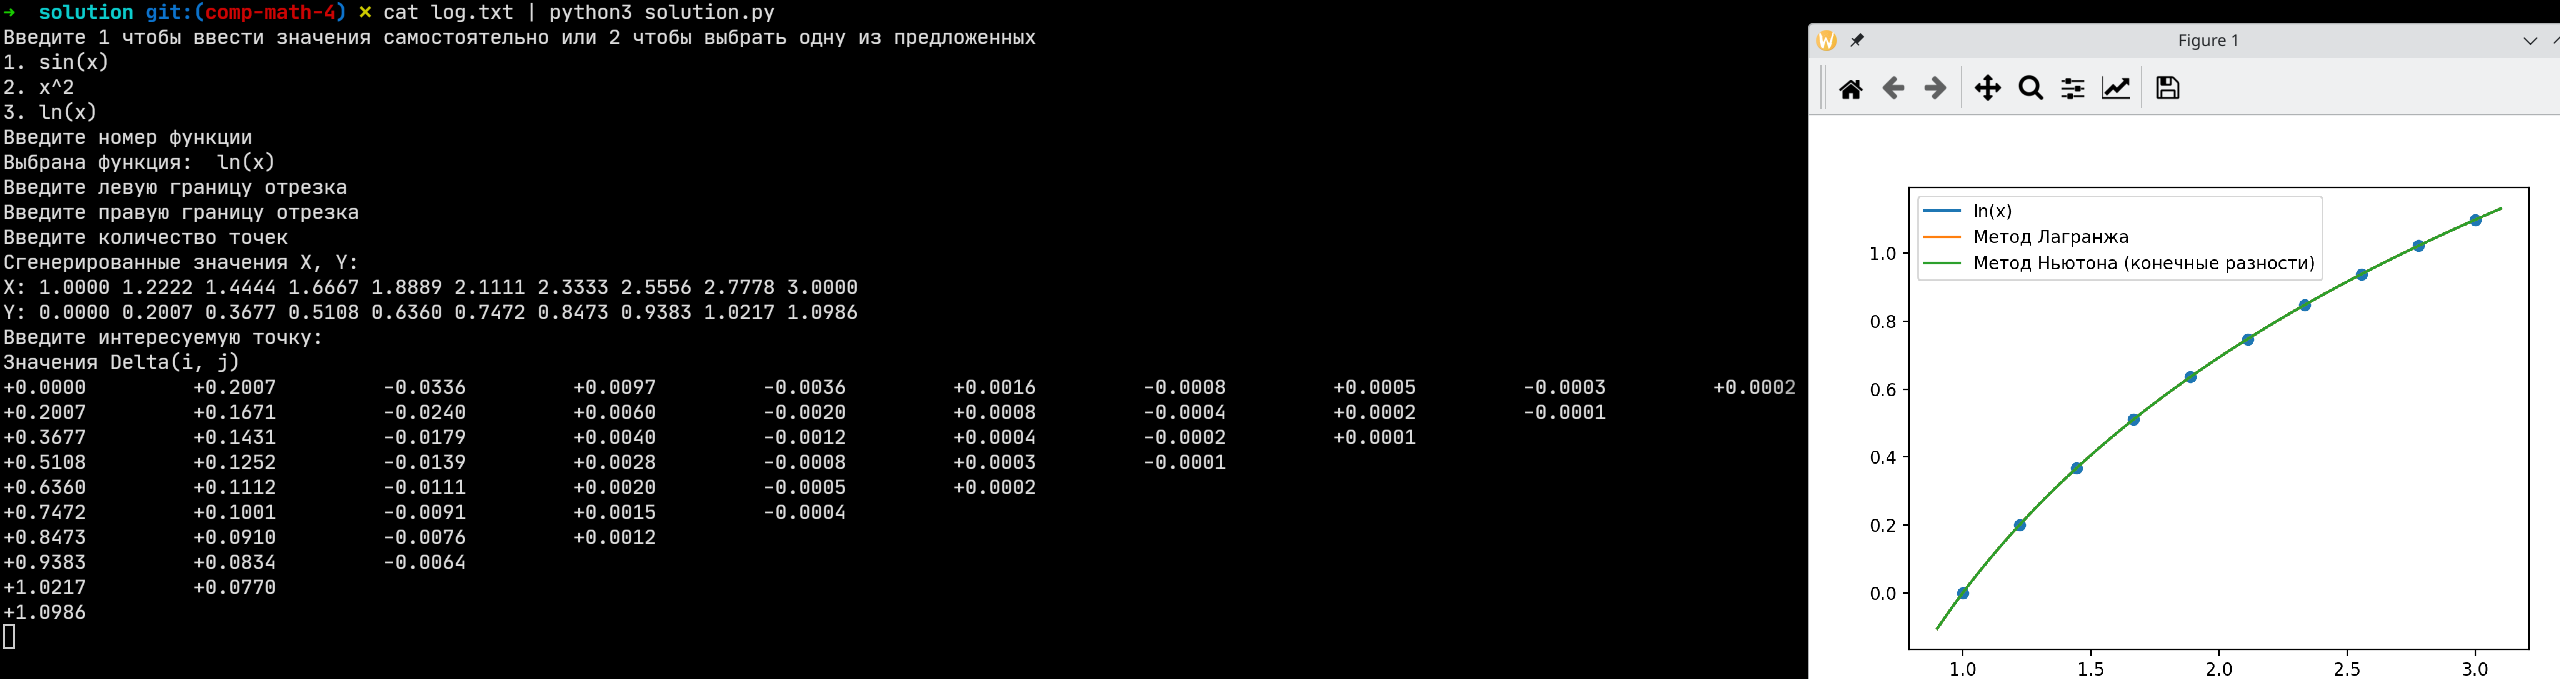
\includegraphics[width=\textwidth]{img/demo1.png}
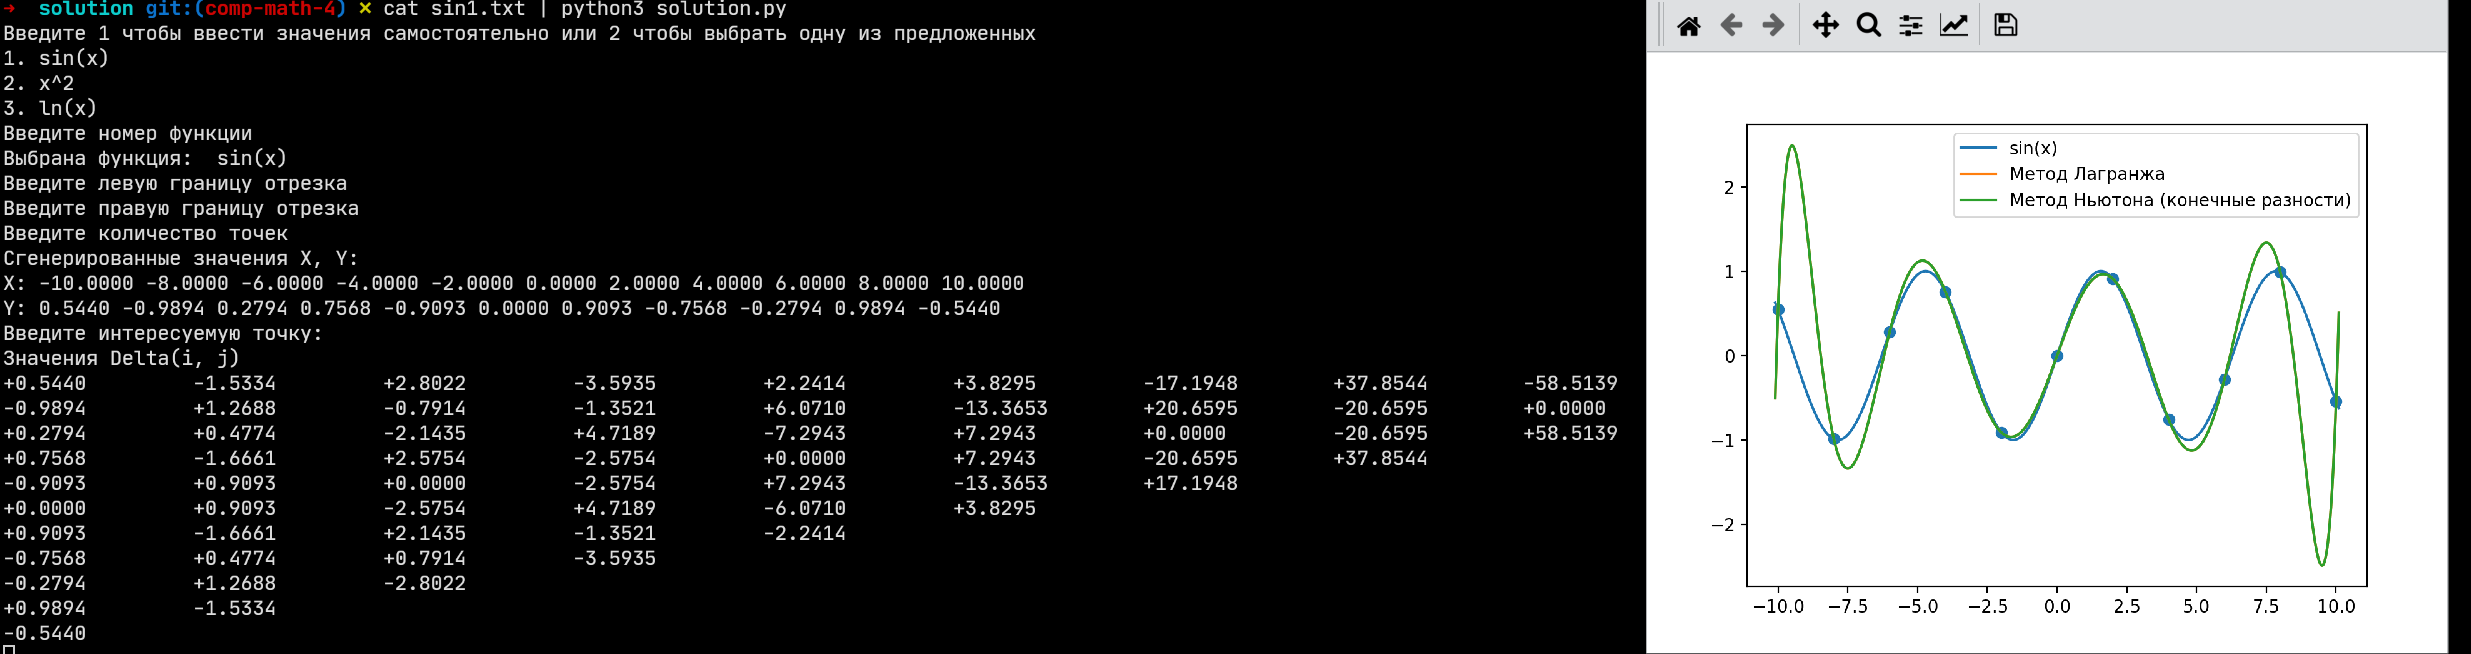
\includegraphics[width=\textwidth]{img/demo2.png}
\end{center}

\section{Вывод}
В ходе выполнения данной лабораторной работы мною были изучены
методы интерполяции Лагранжа, Ньютона и Гаусса.
Эти методы были реализованы на языке программирования Python
а также использованы для вычисления значения функций.
